\section{Introduction}

Lors du HO1, vous avez détecté un son avec un microphone et l'avez filtré pour supprimer sa composante DC. Lors d'un claquement de doigts, le signal obtenu (à la sortie du filtre) reste cependant un signal plutôt complexe: il s'agit d'un signal analogique (il varie de façon continue dans un intervalle de tension, entre un minimum et un maximum), qui oscille plusieurs fois pour un seul claquement de doigts. Tel quel, ce signal est donc difficilement utilisable pour générer un signal de commande propre et stable. Nous allons donc le simplifier:

\begin{enumerate}
    \item Afin qu'il ne prenne comme valeur que \SI{0}{V} ou $V_{DD}$ (la
tension d'alimentation)
    \item Afin qu'il ne comporte qu'une oscillation par évènement sonore.
\end{enumerate}

Le résultat de ces transformations est illustré à la Figure \ref{fig:signal-all}. La transformation (1) se fera au moyen d'un comparateur, et la transformation (2) au moyen d'un circuit intégré NE555 (en mode bascule monostable).

\begin{figure}[h!]
    \centering
    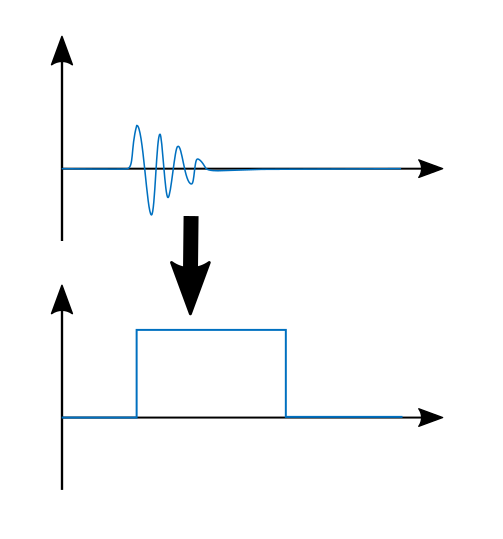
\includegraphics[width=0.5\textwidth]{signals.PNG}
    \caption{Transformation du signal HO2}
    \label{fig:signal-all}
\end{figure}